\documentclass[a4paper,class=article,border=10pt,tikz]{standalone}
\usepackage{tikz}
\usetikzlibrary{snakes,calc,positioning,patterns,angles,quotes,decorations.pathmorphing,decorations.markings,through}
\usetikzlibrary{arrows,decorations,decorations.text}
\usepackage{rotating}
\usetikzlibrary{arrows,decorations,decorations.text}
\usetikzlibrary{patterns.meta,math}




\usepackage{siunitx}

\begin{document}



% two trolleys with 9 connectors for SDOF nonlinear

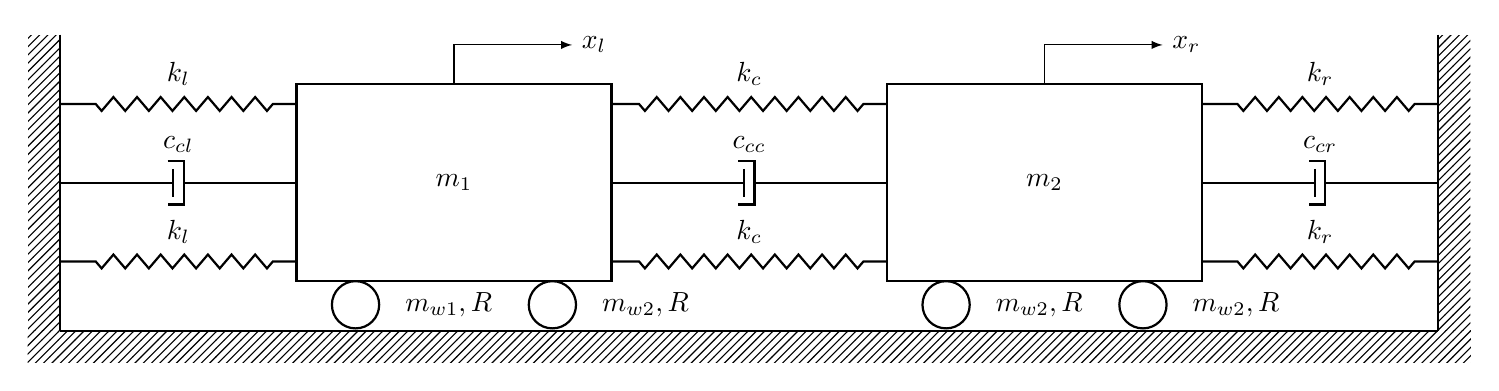
\begin{tikzpicture}
\tikzstyle{spring}=[thick,decorate,decoration={zigzag,pre length=0.3cm,post length=0.3cm,segment length=0.3cm}]
\tikzstyle{damper}=[thick,decoration={markings,  
  mark connection node=dmp,
  mark=at position 0.5 with 
  {
    \node (dmp) [thick,inner sep=0pt,transform shape,rotate=-90,minimum width=15pt,minimum height=3pt,draw=none] {};
    \draw [thick] ($(dmp.north east)+(2pt,0)$) -- (dmp.south east) -- (dmp.south west) -- ($(dmp.north west)+(2pt,0)$);
    \draw [thick] ($(dmp.north)+(0,-5pt)$) -- ($(dmp.north)+(0,5pt)$);
  }
}, decorate]
\tikzstyle{ground}=[fill,pattern=north east lines,draw=none,minimum width=0.75cm,minimum height=0.3cm]

\node (M) [draw,outer sep=0pt,thick,minimum width=4cm, minimum height=2.5cm] {$m_1$};
\node (M2) [draw,outer sep=0pt,thick,minimum width=4cm, minimum height=2.5cm,xshift=7.5cm] at (M) {$m_2$};

%\node (ground) [ground,anchor=north west,xshift=-2.4cm,yshift=-0.25cm,minimum width=17.75cm] at (M.south west) {};
\node (wall_1) [ground,anchor=east,xshift=-3cm,yshift=0cm,minimum height=3.75cm ,minimum width=0.4cm] at (M.west) {};
\node (wall_2) [ground,anchor=west,xshift=3cm,yshift=0cm,minimum height=3.75cm ,minimum width=0.4cm] at (M2.east) {};

\draw[thick] (wall_1.south east) -- (wall_2.south west);
\draw[thick] (wall_1.north east) -- (wall_1.south east);
\draw[thick] (wall_2.north west) -- (wall_2.south west);
\draw[ground] (wall_2.south east)++(0,-0.4cm)  rectangle (wall_1.south west);


\draw [thick] (M.south west) ++ (0.75cm,-0.3cm) circle (0.3cm) node[right=0.5cm] {$m_{w1},R$}  (M.south east) ++ (-0.75cm,-0.3cm) circle (0.3cm) node[right=0.5cm] {$m_{w2},R$};
\draw [thick] (M2.south west) ++ (0.75cm,-0.3cm) circle (0.3cm) node[right=0.5cm] {$m_{w2},R$}  (M2.south east) ++ (-0.75cm,-0.3cm) circle (0.3cm) node[right=0.5cm] {$m_{w2},R$};

\draw [damper]  (M2.180) ++ (0cm,0cm) -- ($ (M.0 )+(0cm,0cm)  $)  node [pos=0.5,above=0.25cm] (k_cc) {$c_{cc}$};
%\draw [fill=black]  (M2.180) ++ (0cm,0.15cm) rectangle ($ (M.0 )+(0cm,-0.15cm)  $) ;

\draw [damper]  (M.180) ++ (0cm,-0.0cm) -- ($ (wall_1.0 )+(0cm,0.0cm)  $) node [pos=0.5,above=0.25cm](k_cl) {$c_{cl}$};
%\draw [fill=black]  (M.180) ++ (0cm,0.15cm) rectangle ($ (wall_1.0 )+(0cm,-0.15cm)  $) ;

\draw [damper]  (wall_2.180) ++ (0cm,0cm) -- ($ (M2.0 )+(0cm,0cm)  $)node [pos=0.5,above=0.25cm] (k_cr) {$c_{cr}$};
%\draw [fill=black]  (wall_2.180) ++ (0cm,0.15cm) rectangle ($ (M2.0 )+(0cm,-0.15cm)  $) ;



\draw [spring]  (M2.180) ++ (0cm,1cm) -- ($ (M.0 )+(0cm,1cm)  $)  node [pos=0.5,above=0.10cm] (k_c) {$k_c$};
\draw [spring]  (M.180) ++ (0cm,1cm) -- ($ (wall_1.0 )+(0cm,1cm)  $) node [pos=0.5,above=0.10cm](k_l) {$k_l$};
\draw [spring]  (wall_2.180) ++ (0cm,1cm) -- ($ (M2.0 )+(0cm,1cm)  $)node [pos=0.5,above=0.10cm] (k_r) {$k_r$};


\draw [spring]  (M2.180) ++ (0cm,-1cm) -- ($ (M.0 )+(0cm,-1cm)  $)  node [pos=0.5,above=0.10cm] (k_c) {$k_c$};
\draw [spring]  (M.180) ++ (0cm,-1cm) -- ($ (wall_1.0 )+(0cm,-1cm)  $) node [pos=0.5,above=0.10cm](k_l) {$k_l$};
\draw [spring]  (wall_2.180) ++ (0cm,-1cm) -- ($ (M2.0 )+(0cm,-1cm)  $)node [pos=0.5,above=0.10cm] (k_r) {$k_r$};


\draw [-latex,thin] (M.north) --++ (0cm,0.5cm) -- +(1.5cm,0cm) node[right] {$x_l$};
\draw [-latex,thin] (M2.north) --++ (0cm,0.5cm) -- +(1.5cm,0cm) node[right] {$x_r$};


% \draw [thin] (M.north) --++ (0cm,1cm) node (f_l_start) {}  --+ (1.5cm,0cm) node[right] (f_l_end) {$F_0 \cos(\Omega t)$};
% \draw [-latex,thick]  (f_l_start.center)  --(f_l_end.west);

% \draw [thin] (M2.north) --++ (0cm,1cm) node (f_p_start) {} --+  (1.5cm,0cm) node[right] (f_p_end) {$F_0 \cos(\Omega t)$};
% \draw [-latex,thick]  (f_p_start.center)  -- (f_p_end.west);

\end{tikzpicture}




\end{document}